\section{The background measurement campaign}
\label{sec:Measurement}

%Using two 30 X 30 X 2\cm wrapped plastic scintillators with photomultiplier tube (PMT) attached on iron test stand. 
%Each PMTs receives 1.5 kV high voltage and 350 V bias voltage. 
%Why do we set high voltage to 1.5 kV? Because rate increases with bigger high voltage, but it becomes flat when high voltage larger than 1.5 kV
%The scintillators measure mininum ionizing particles (mip).
%This supports by NIM crate.
%We test this equipments at lab taking cosimc rays
%This is the first time measured hit rate at underground cavern.
%Results from measurments may impact to other LLP experiments.
%When particle goes through scintillators and makes hits on both detectors, we counts number of events. 
%We made 30 mV threshold of signal pick to measure data which has physical meaning. 
%Triggering when signals appear at both detector in 5 ns. 
%Since detector have been placed 100 m below underground, muons from cosmic rays decay are suppressed. 
%We take data during MD and when the beam is online. 
%We switch the detector position several times. Also we take data while detector is rotated. 
%This is the first measurement of hit rate at D3 platform. 
%We use scope to take data, hit rate is not high. 
%We remotely connect to scope and able to manage scope.
%We took data from 4 different places. 
%Back of D3 platform of each corner and central position.
%Front D3 platform at central with parallel to beam line and make 45 degree with a beam line.





\begin{figure}
\centering
\subfigure[]{
\centering
   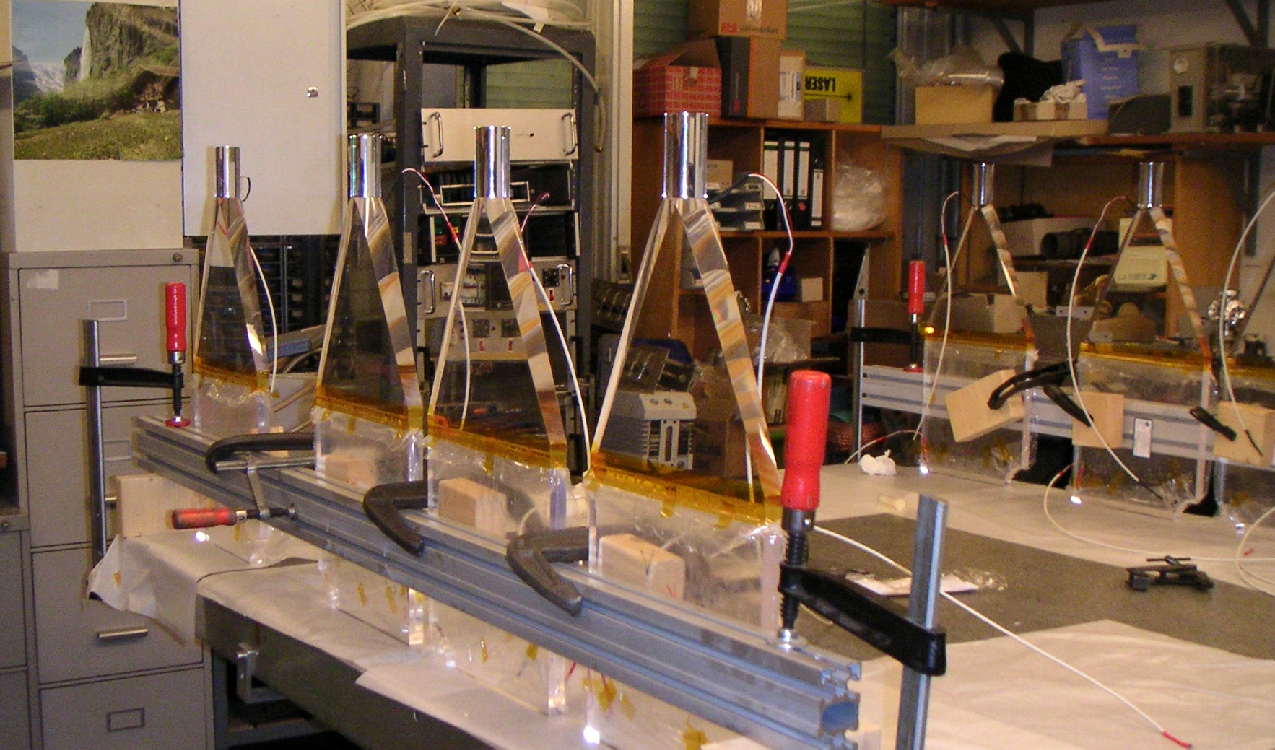
\includegraphics[width=0.47\columnwidth]{figs/INT/codexb_scin_assembly.pdf}
}
\subfigure[]{
\centering
   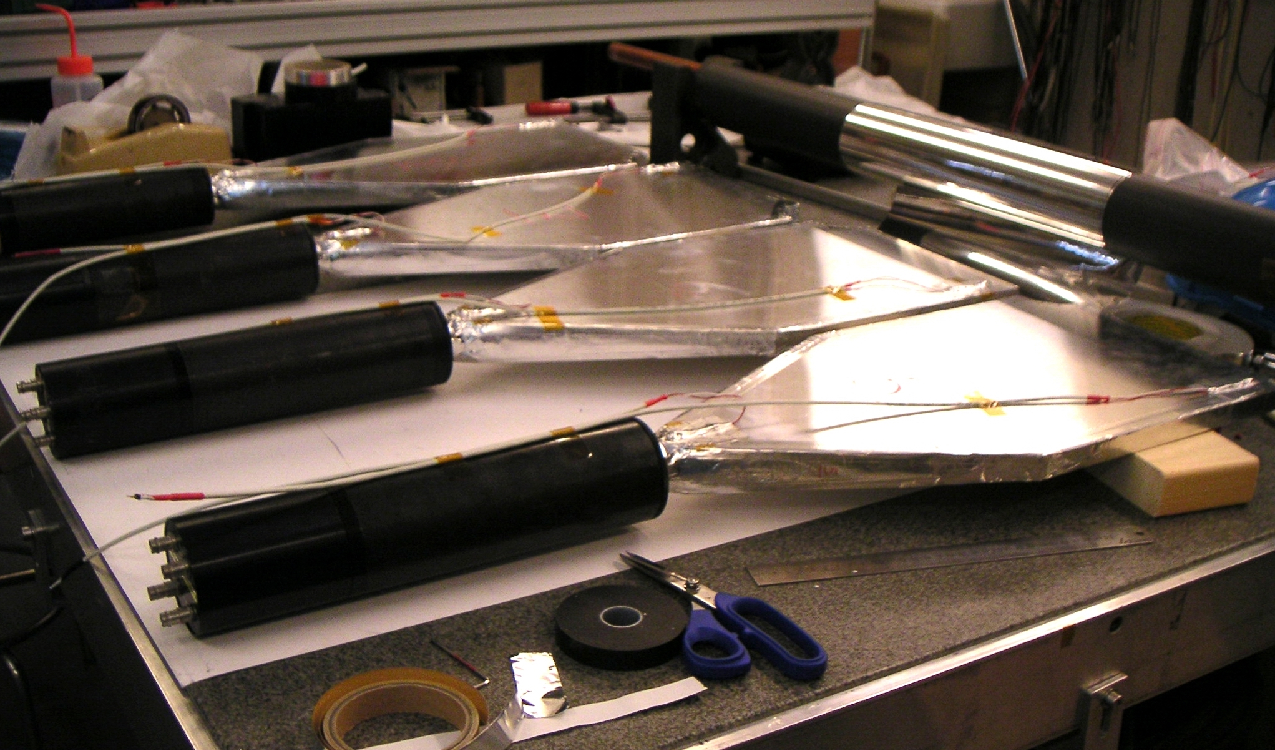
\includegraphics[width=0.47\columnwidth]{figs/INT/codexb_scin_wrapping.pdf} 
}
\caption{\label{fig:scint}
HeRSCheL scintillators: (a) scintillator and light-guide assembly, (b) wrapped scintillators coupled to the PMT in the casing with additional electronics.
}
\end{figure}

\subsection{Scintillator, PMT and the test bench}
The measurement setup re-uses scintillators, light-guides and photomultiplier tubes (PMT) taken from the HeRSCheL detector~\cite{LHCb-DP-2016-003} in LHCb. The plastic scintillating material is EJ-200 ($300\times300\times20$~mm$^3$) and light-guides providing the coupling to the PMT is made of Plexiglass. The scintillator and light-guide are wrapped in light-protecting aluminium foil. Each light guide is coupled to a Hamamatsu R1828-01 PMT chosen due to its high anode current upper limit, wide range of gain variation, fast time response to fit in 25~ns, large entry window for enhanced light yield and good single electron separation. Figure~\ref{fig:scint} shows the scintillator-PMT assembly~\cite{LHCb-DP-2016-003}.


\begin{figure}
\centering
\subfigure[]{
\centering
   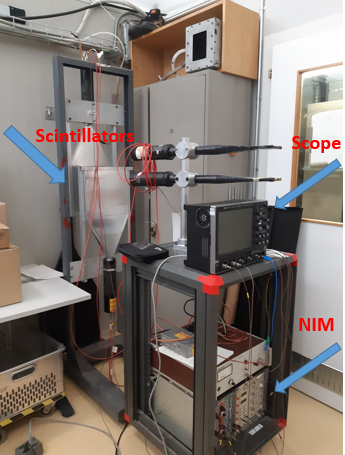
\includegraphics[width=0.47\columnwidth]{figs/INT/Tools.png}
}
\subfigure[]{
\centering
   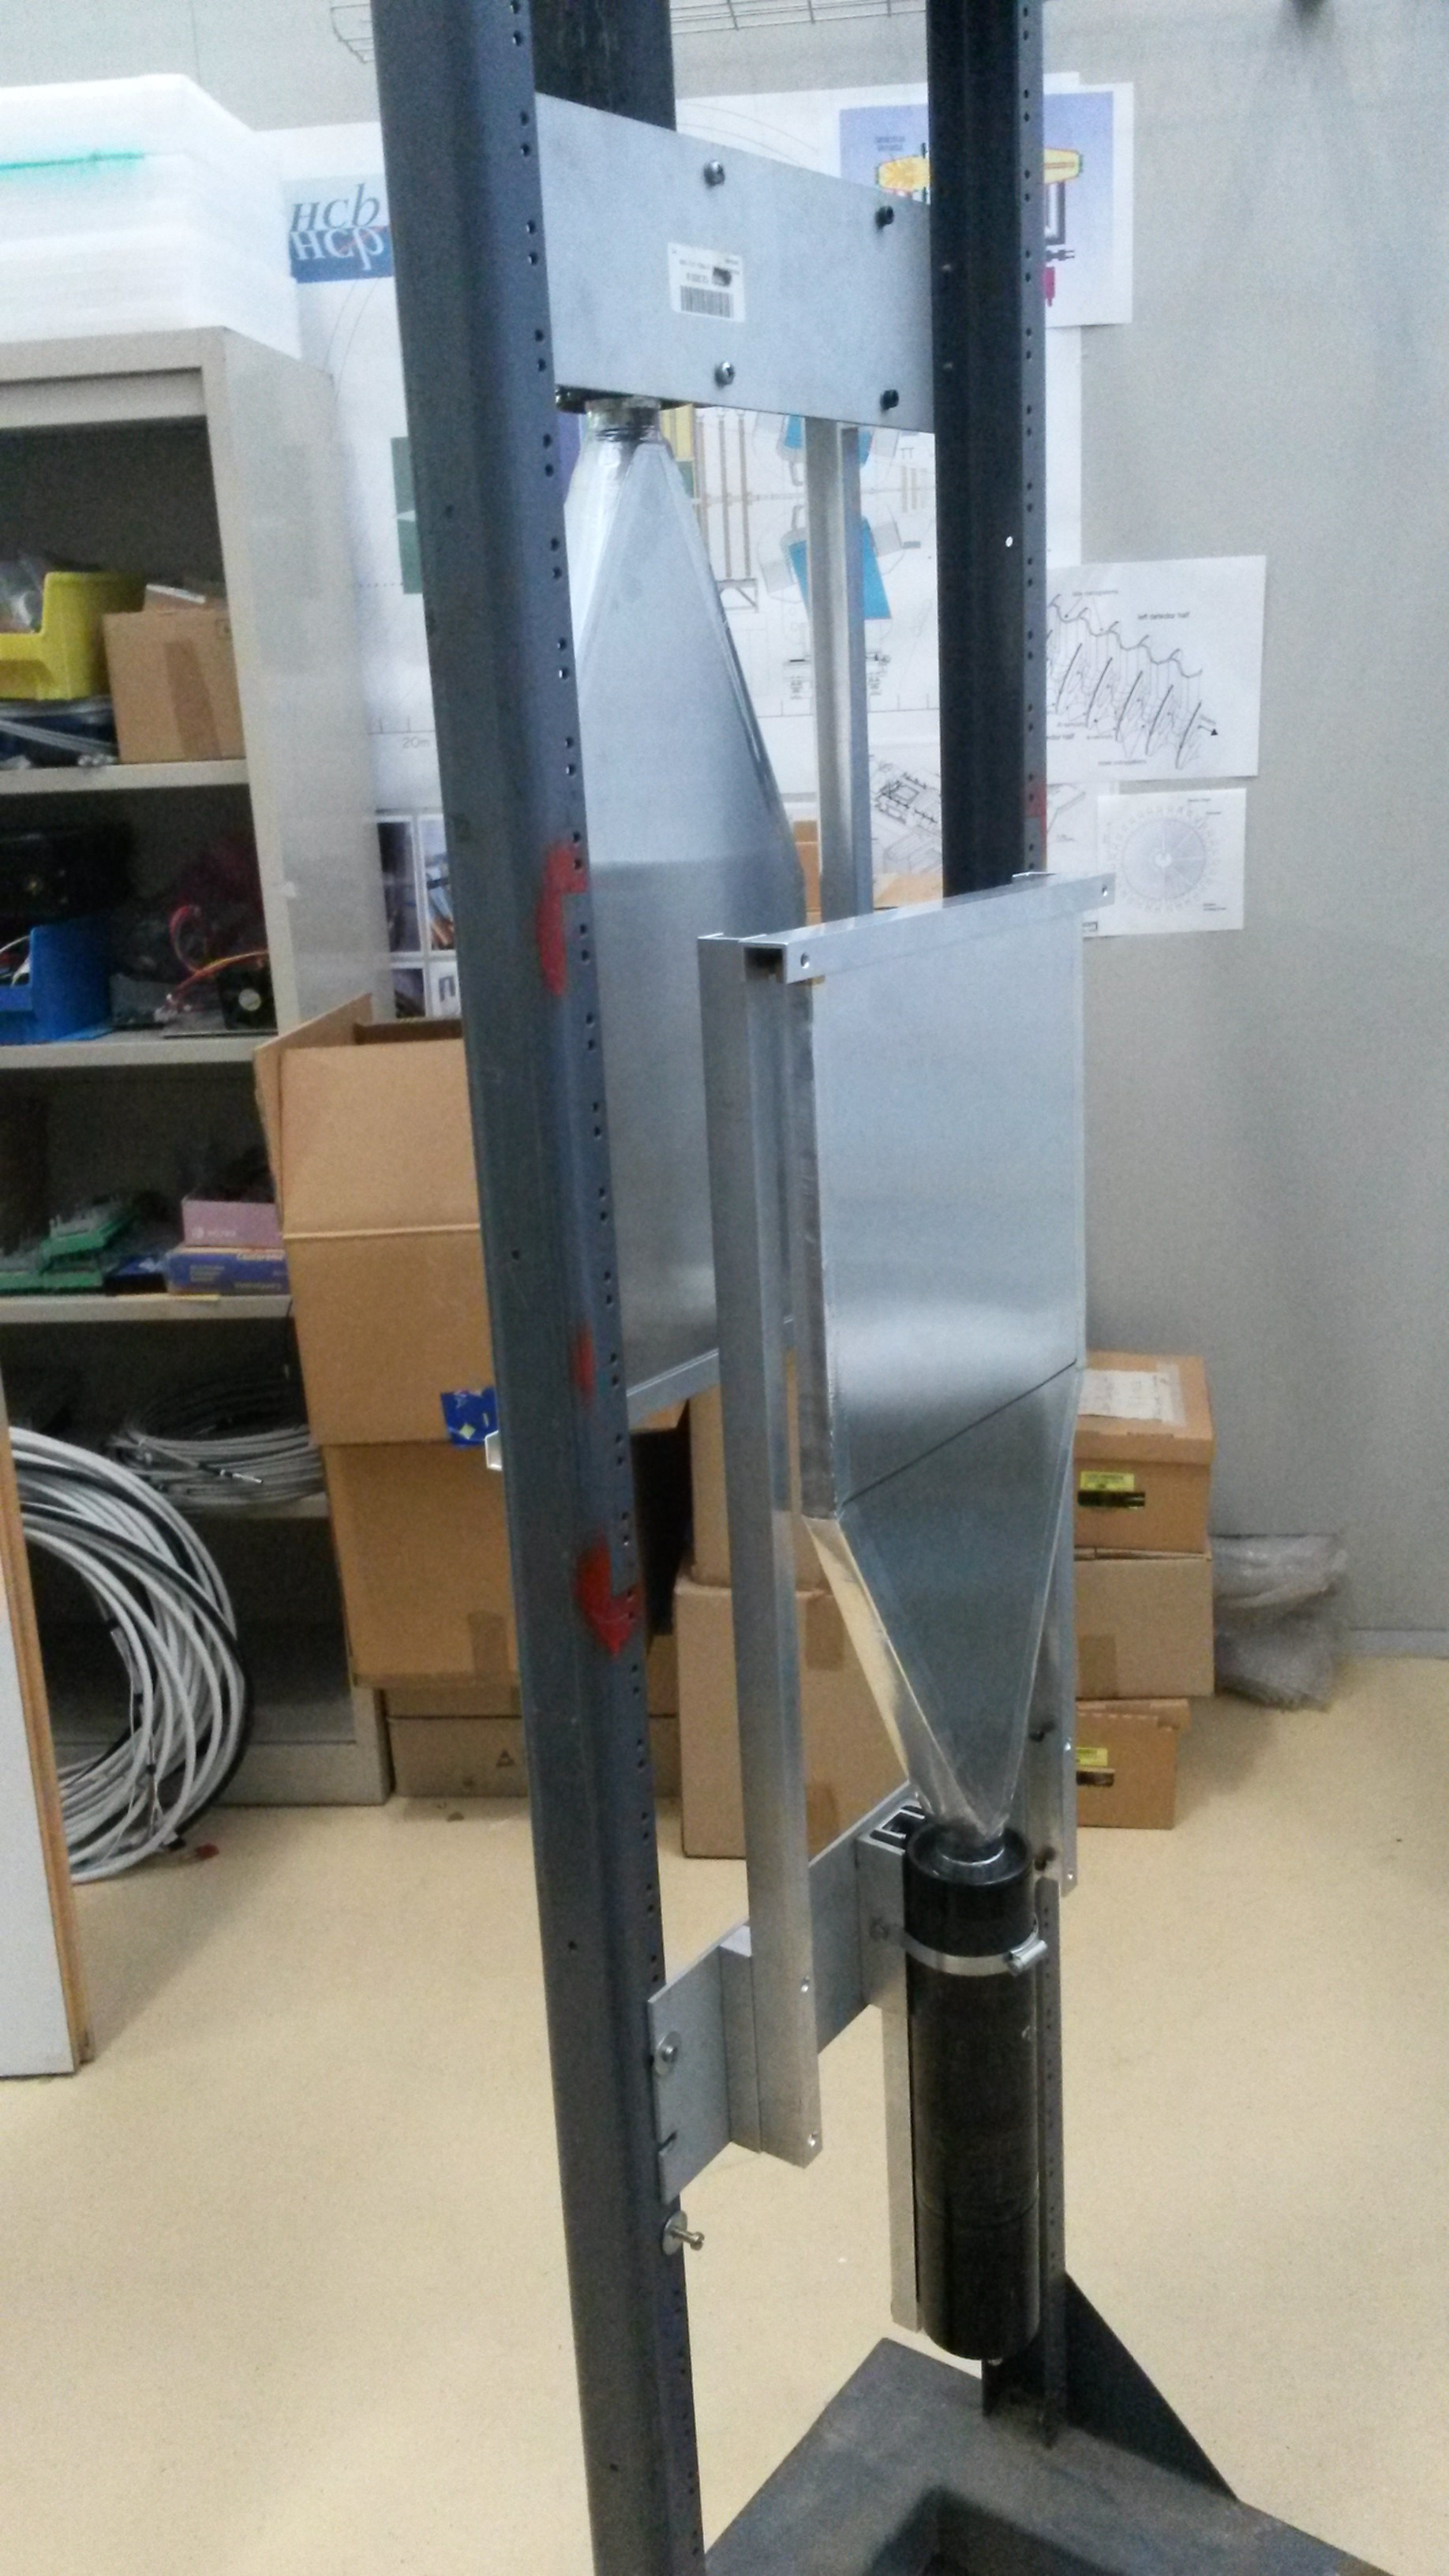
\includegraphics[width=0.34\columnwidth]{figs/INT/mechanical_stand_1.jpg} 
}
\caption{\label{fig:test_bench} Test-bench assembly in the VeloPix lab showing the (a) HeRSCheL scintillators, the DAQ system comprising a NIM crate and oscilloscope. The cosmic stand used for initial tests is also shown, (b) close-up look at the mechanical stand.
}
\end{figure}

Figure~\ref{fig:test_bench} shows the test bench assembly in the lab. It includes a vertical iron mechanical stand holding the wrapped scintillator pair and the NIM crate power supply providing -1.5kV HV, with an additional -350V bias voltage. The horizontal distance between the two scintillators is 2~cm. The DAQ system utilized an oscillosscope (LeCroy WaveRunner) with extended functions (autosave waveforms, coincidence logic, etc). Before transporting the setup to Point~8, it was tested with a cosmic stand also shown in Fig.~\ref{fig:test_bench}. 


\subsection{Trigger}
We use a simple 2-fold coincidence between the two scintillators, with a discrimination threshold set as 30~mV on the oscilloscope. The time-window for the coincidence is 5~ns. The scope automatically saves two waveforms from each scintillator, as shown in Fig.~\ref{fig:waveform}, along with the timestamp, for every mip )minimum ionising particle) hit event (not to be confused with collision events). This timestamp is important to correlate with the beam status during data-taking.

\begin{figure}
\centering
    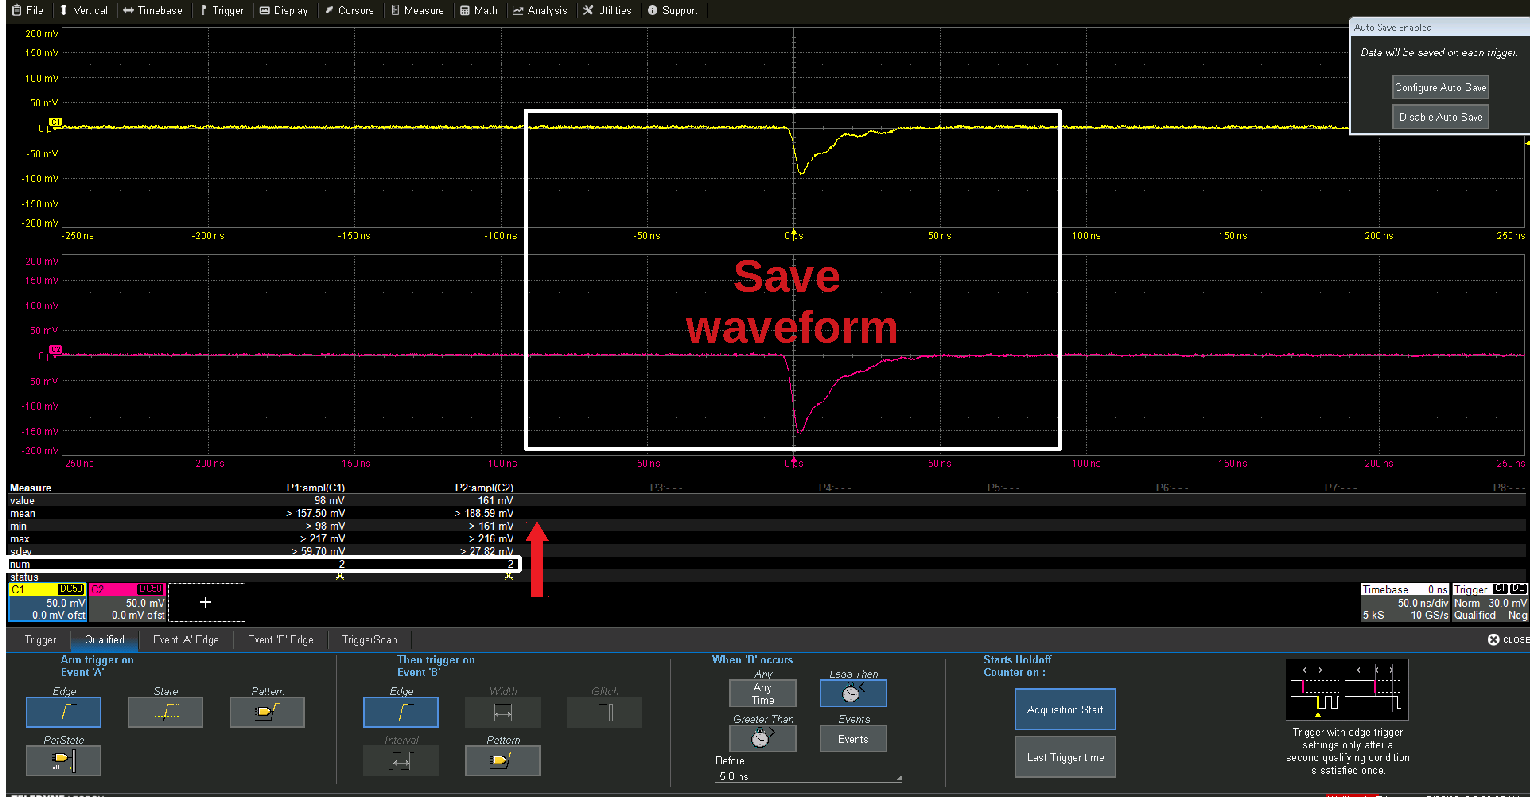
\includegraphics[width=16cm]{figs/INT/waveform.pdf}
\caption{\label{fig:waveform}
    Trigger setup using coincidence occurence of signals from the two scintillator PMT's within 5~ns. 
}
\end{figure}

\subsection{Measurement positions and configurations on the D3 platform}

\begin{figure}
\centering
    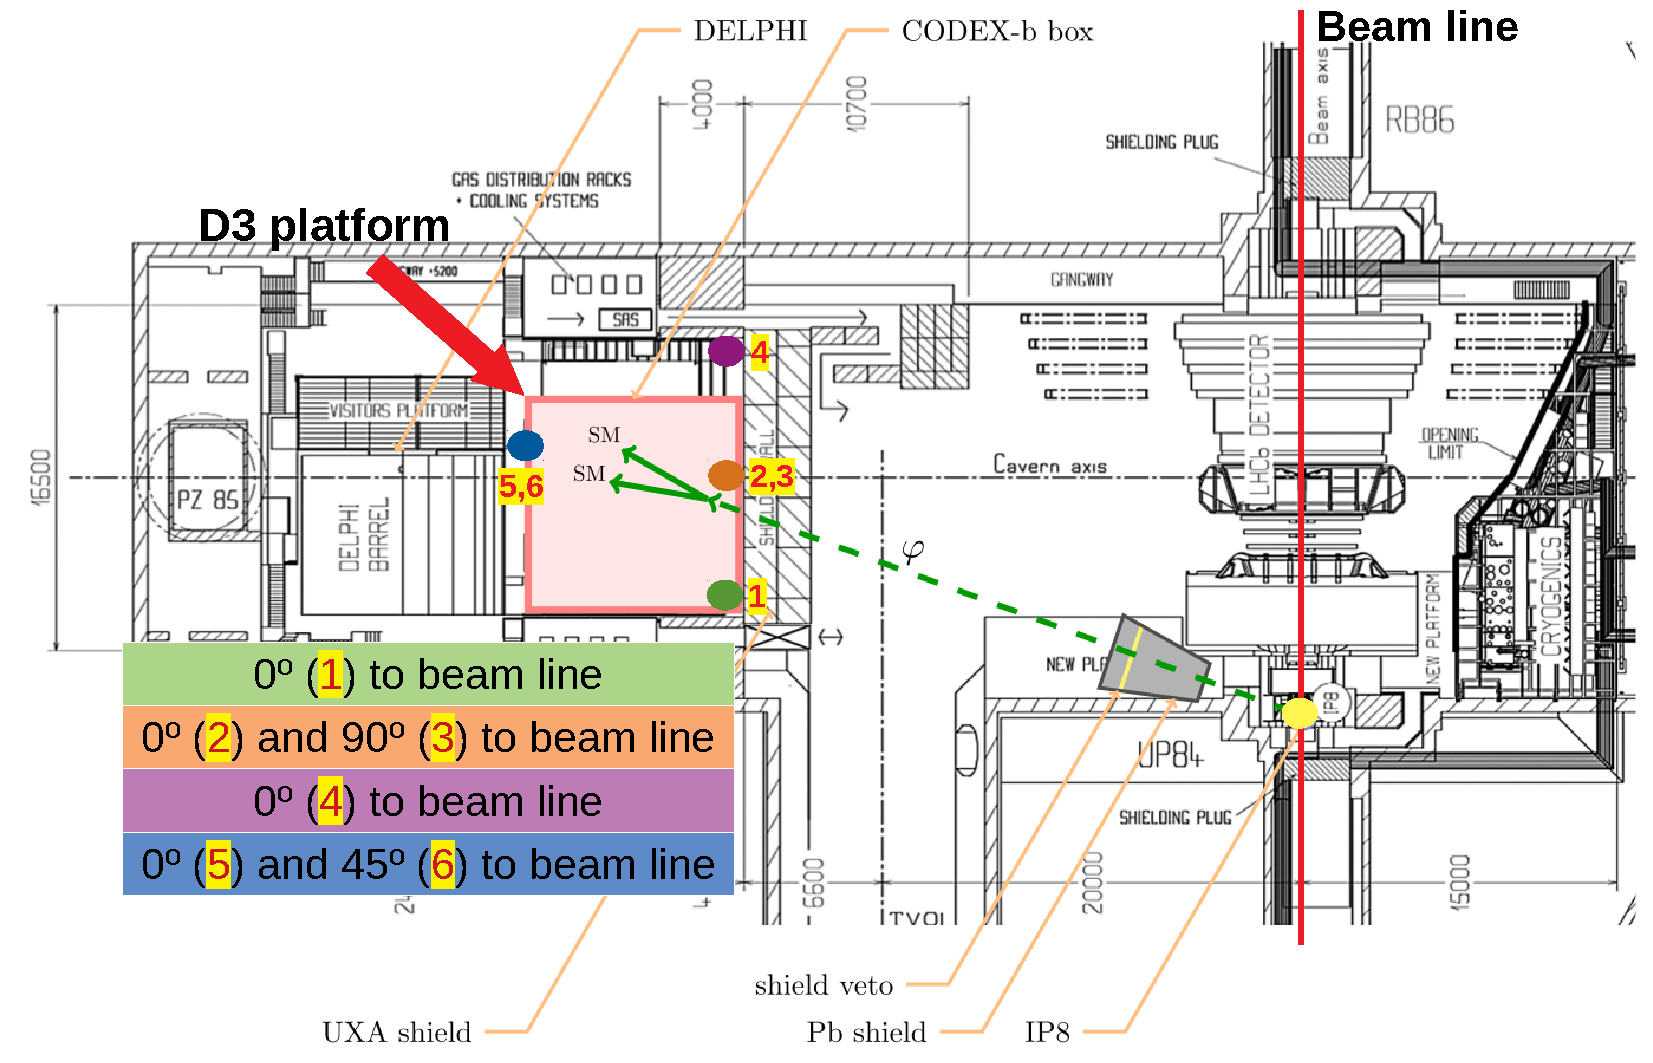
\includegraphics[width=16cm]{figs/INT/configuration.pdf}
\caption{\label{fig:posconfig}
    The four measurement positions on the D3 level inside the LHCb cavern. The configurations are labelled from P1-P6.
}
\end{figure}


\begin{figure}
\centering
\subfigure[]{
\centering
   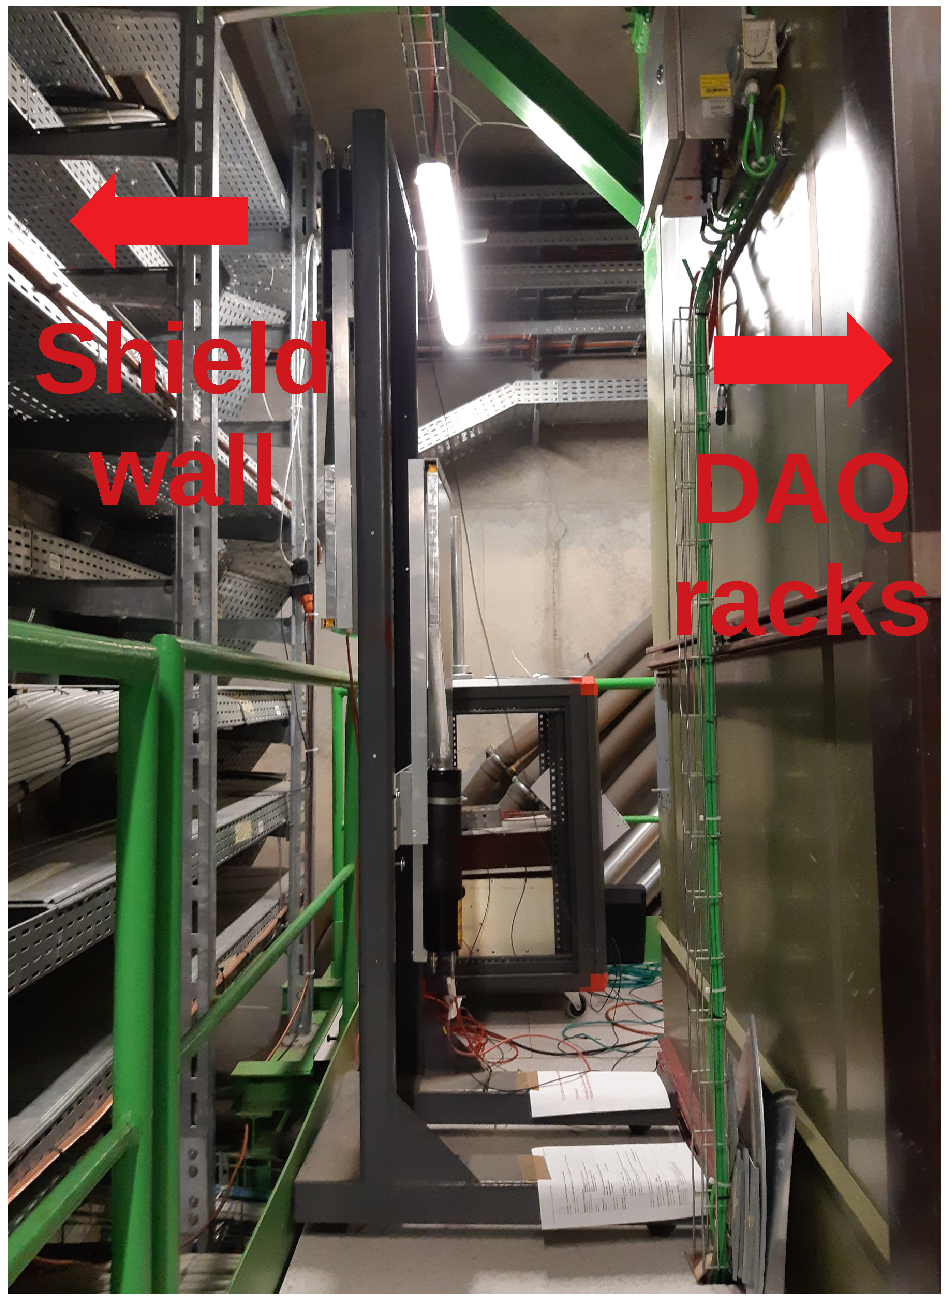
\includegraphics[width=0.4\columnwidth]{figs/INT/Initial.pdf} 
}
\subfigure[]{
\centering
   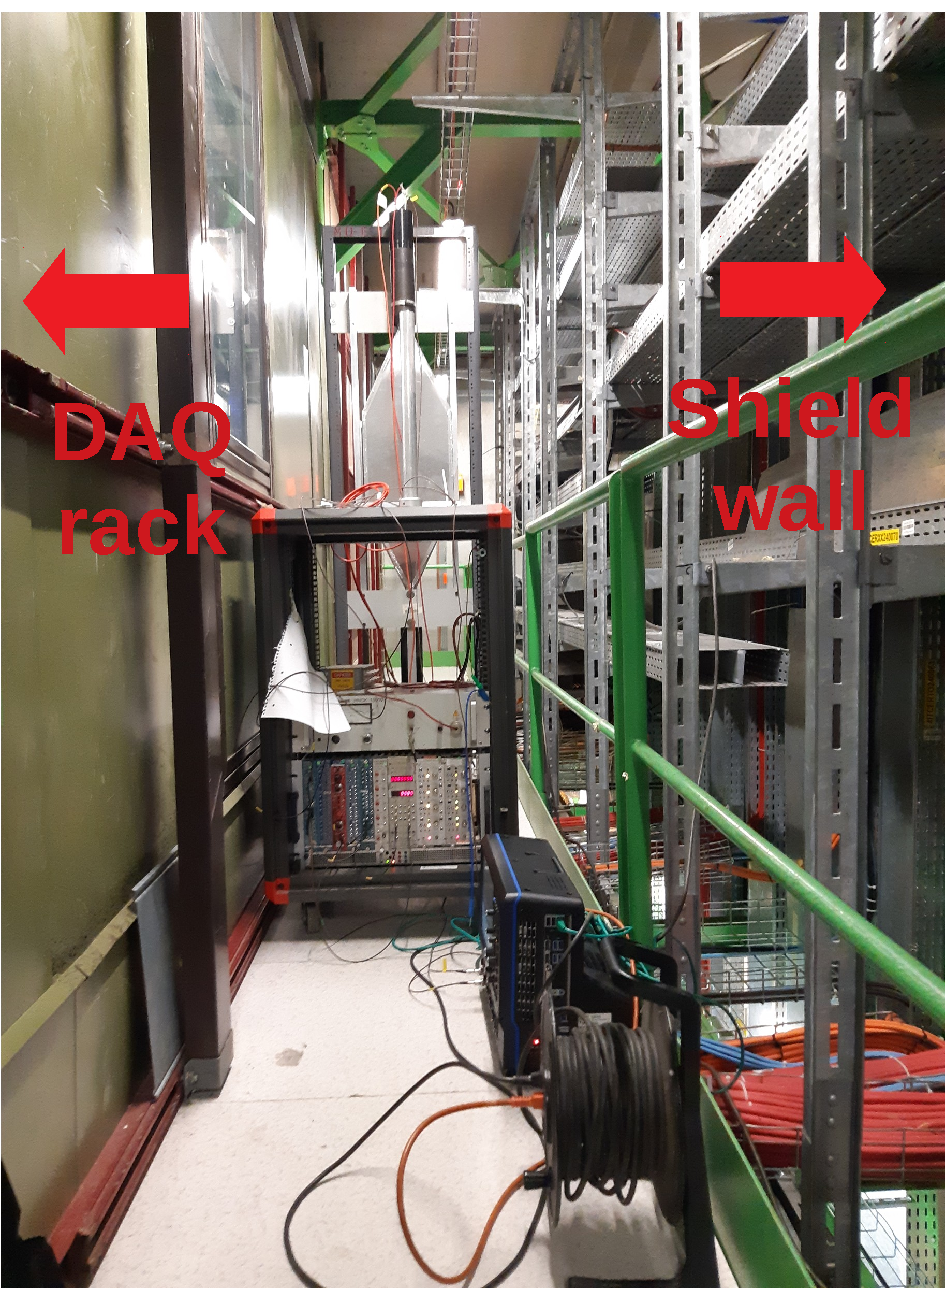
\includegraphics[width=0.4\columnwidth]{figs/INT/Back_central.pdf}
}
\subfigure[]{
\centering
   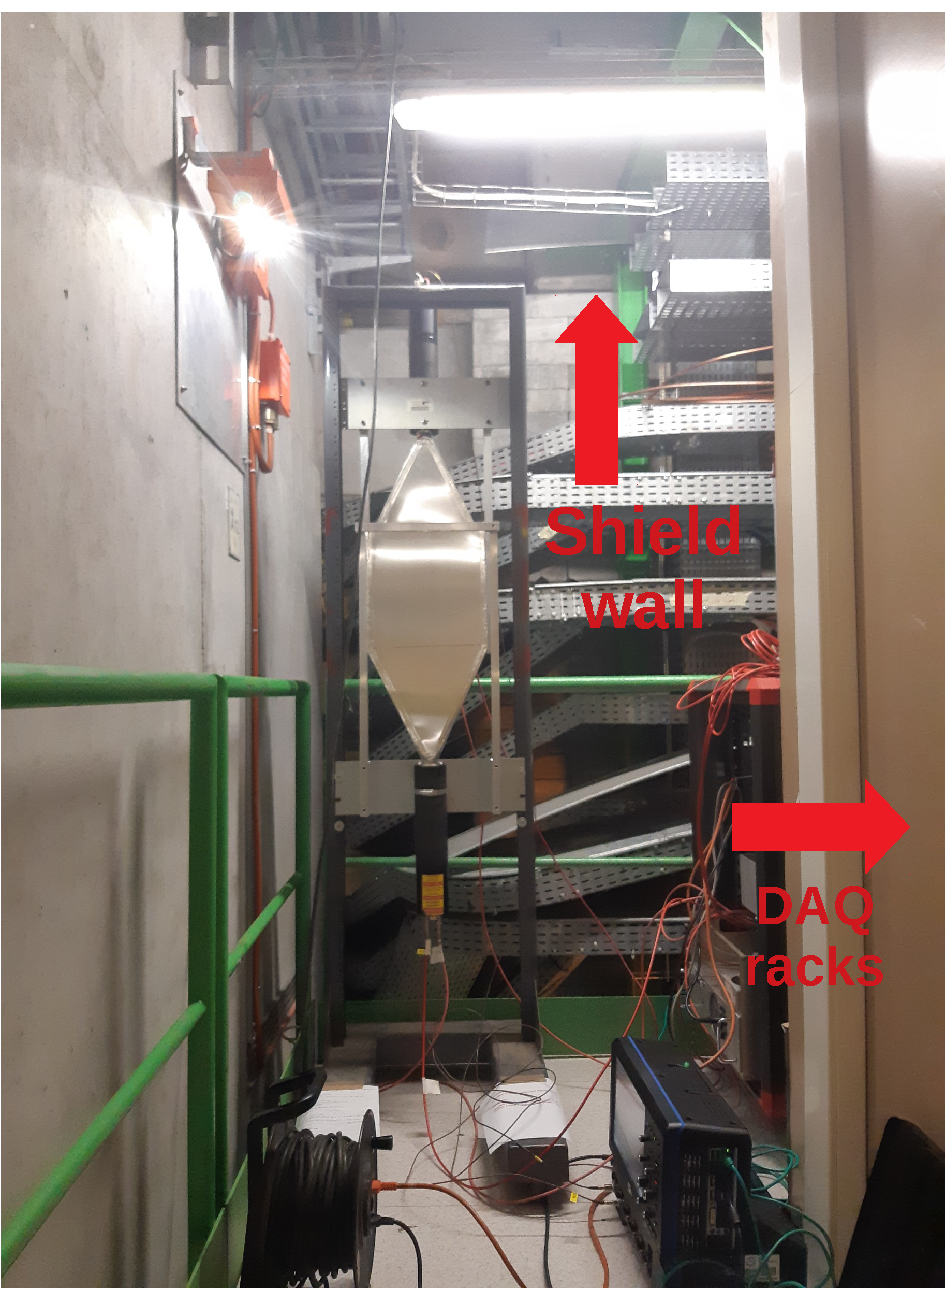
\includegraphics[width=0.4\columnwidth]{figs/INT/Othercorner.pdf} 
}
\subfigure[]{
\centering
   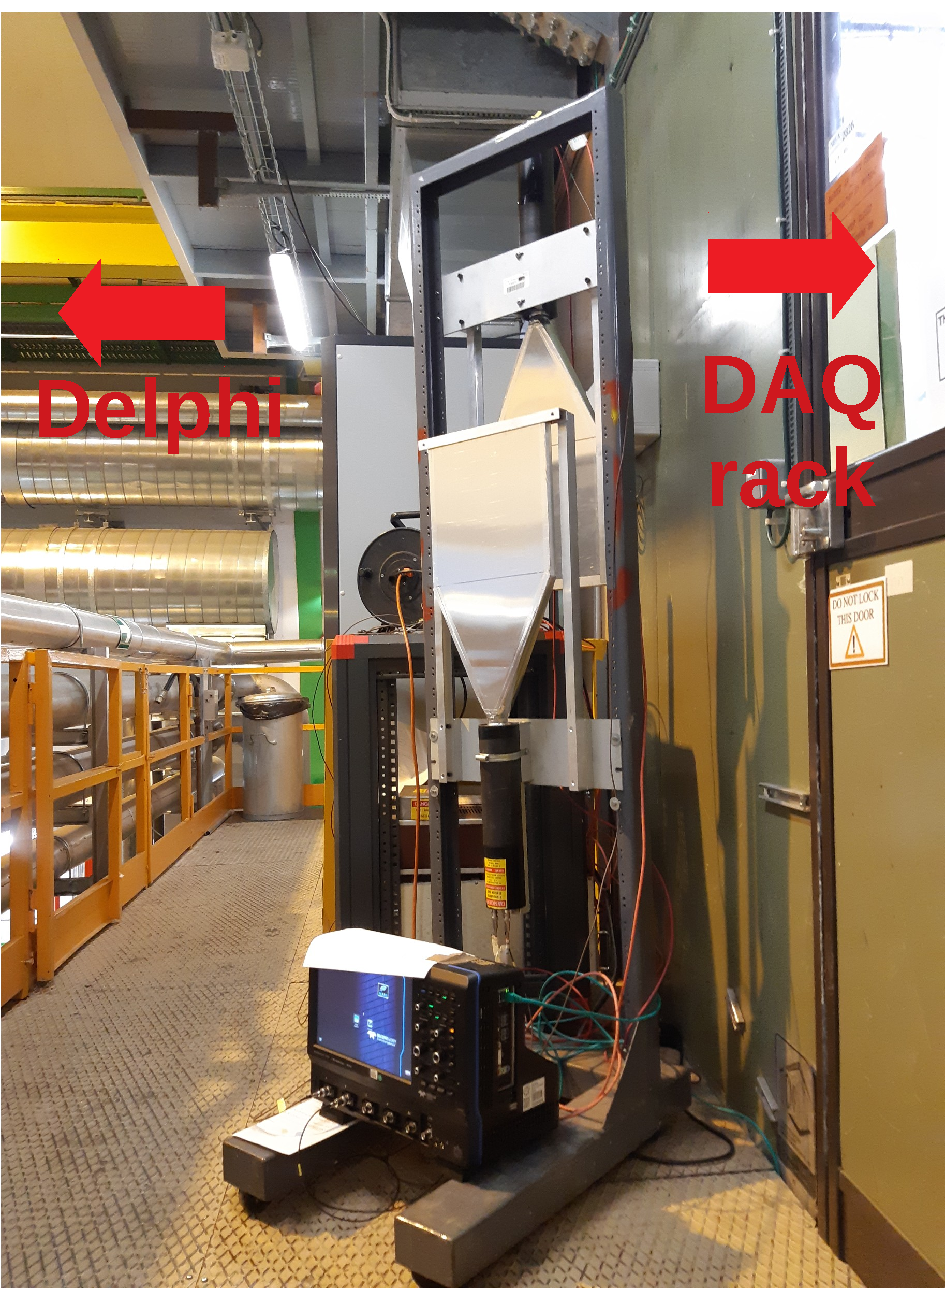
\includegraphics[width=0.4\columnwidth]{figs/INT/D3_front.pdf} 
}
\caption{\label{fig:det_equip}
    Photos of the equipment setup at various positions on the D3 platform: (a) P1, (b) P3, (c) P4, and (d) P6.
}
\end{figure}

The background measurements were taken in the LHCb cavern on D3 platform level, just behind the concrete shield wall, on the access side. The equipment was set up at 3 positions on the passarelle between DAQ racks and the concrete shield wall, one position between the \delphi exhibit and DAQ racks. For orientation, the scintillator stand was mostly parallel to the beam line but was also rotated $45^{\circ}$ and perpendicular to the beam line. Figure~\ref{fig:posconfig} shows the positions and configurations for the measurements, and Fig.~\ref{fig:det_equip} shows pictures of the equipment at these positions on the D3 platform.


\subsection{Results}

\begin{figure}
\centering
    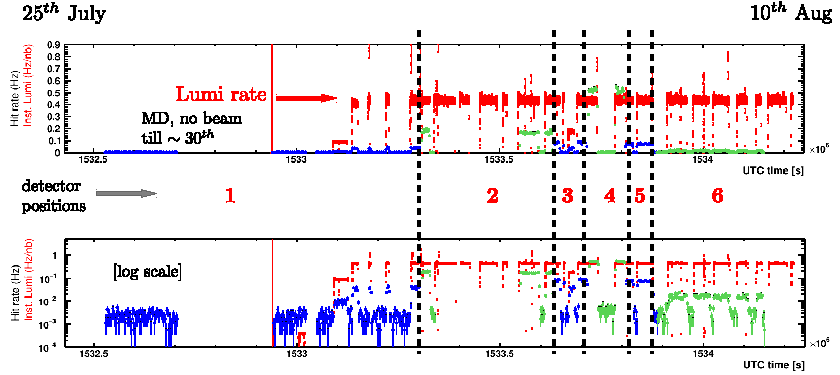
\includegraphics[width=16cm]{figs/INT/codexb_data_global.pdf}
\caption{\label{fig:results} The Hit rate plots during the run based on 6 positions/configurations linear and log scale. Red dots mean the lumi rate of \lhcb, blue and green dots mean hit rates. The results are not officially approved by the LHCb collaboration.
}
\end{figure}

The measurement campaign spanned over 17 days between $25^{th}$ July and $10^{th}$ August, 2018. There were 52,036 recorded triggers during the run.The LHCb instantaneous luminosity rate was stable during the measurement. There was no beam till July 30th because of machine development and an inadvertent power loss happened during this initial phase. Figure~\ref{fig:results} show the main results from the measurement campaign. The red dots correspond to the instantaneous luminosity measured by LHCb in Hz/nb. The green and blue dots show the hit rate in Hz, alternating between the 6 different configurations/positions, for better visibility. The plots are shown in both normal and logarithmic scales.


\begin{table}
\begin{center}
\begin{tabular}{c|l|r}
  Position & \hspace{2cm}Description & Hit rate [mHz] \\
  \hline \hline
   P1 & shield, right corner, $\parallel$ to beam& $1.99\pm0.07$ \\ \hline
   P2 & shield, center, $\parallel$ to beam&  $2.76\pm 0.03$ \\ \hline
   P3 & shield, center, $\perp$ to beam& $ 2.26\pm 0.03$ \\ \hline
   P4 & shield, left corner, $\parallel$ to beam& $ 3.11\pm 0.03$ \\ \hline
   P5 & shield + D3 racks, center, $\parallel$ to beam& $ 1.95\pm 0.03$ \\ \hline
   P6 & shield + D3 racks, center, $45^\circ$ to beam& $ 2.22\pm $ 0.02\\ \hline
\end{tabular}
\caption{\label{table:rate_no_beam}
    Background hit rates based on each configuration when the beam is off.
}
\end{center}
\end{table}

Table~\ref{table:rate_no_beam} lists the hit rate from ambient background in between fills or during MD, without beam. The average hit rate at each position and configuration is 2~mHz.  THis indicates that the ambient background can be considered negligible for this measurement. Table~\ref{table:rate_stable_beam} lists the hit rate during stable beam. The rate is non-negligible, even for a small area of $300\times300$~mm$^2$. The rate increases from P1$\to$P2$\to$P4, which, from Fig.~\ref{fig:posconfig} indicates that the downstream region sees more activity. This dependence on the $\eta$ has to be corroborated with the simulation. Further, comparing the rate at P2 with P5, behind the DAQ racks, the racks are seen to add shield material. Finally, comparing the rate at P5 and P6, for the angular scan, the flux depends on the orientation with respect to the beam direction, as expected. 

\begin{table}
\begin{center}
\begin{tabular}{c|l|r}
  Position & \hspace{0.9cm}Description & Hit rate [mHz] \\
  \hline \hline
   P1 & shield, right corner, $\parallel$ to beam & $ 38.99 \pm 0.99 $\\ \hline
   P2 & shield, center, $\parallel$ to beam& $ 167.10 \pm 1.43$ \\ \hline
   P3 & shield, center, $\perp$ to beam& $ 82.81 \pm 1.55 $ \\ \hline
   P4 & shield, left corner, $\parallel$ to beam& $ 517.45 \pm 3.52 $ \\ \hline
   P5 & shield + D3 racks, center, $\parallel$ to beam& $ 73.58 \pm 1.18 $ \\ \hline
   P6 & shield + D3 racks, center, $45^\circ$ to beam& $ 15.71 \pm 0.33 $ \\ \hline
\end{tabular}
\caption{\label{table:rate_stable_beam}
    Average hit rates measured during stable beam, at various configurations.
}
\end{center}
\end{table}





%\begin{figure}[h]
%  \begin{center}
%    \begin{tabular}[t]{cc}
%      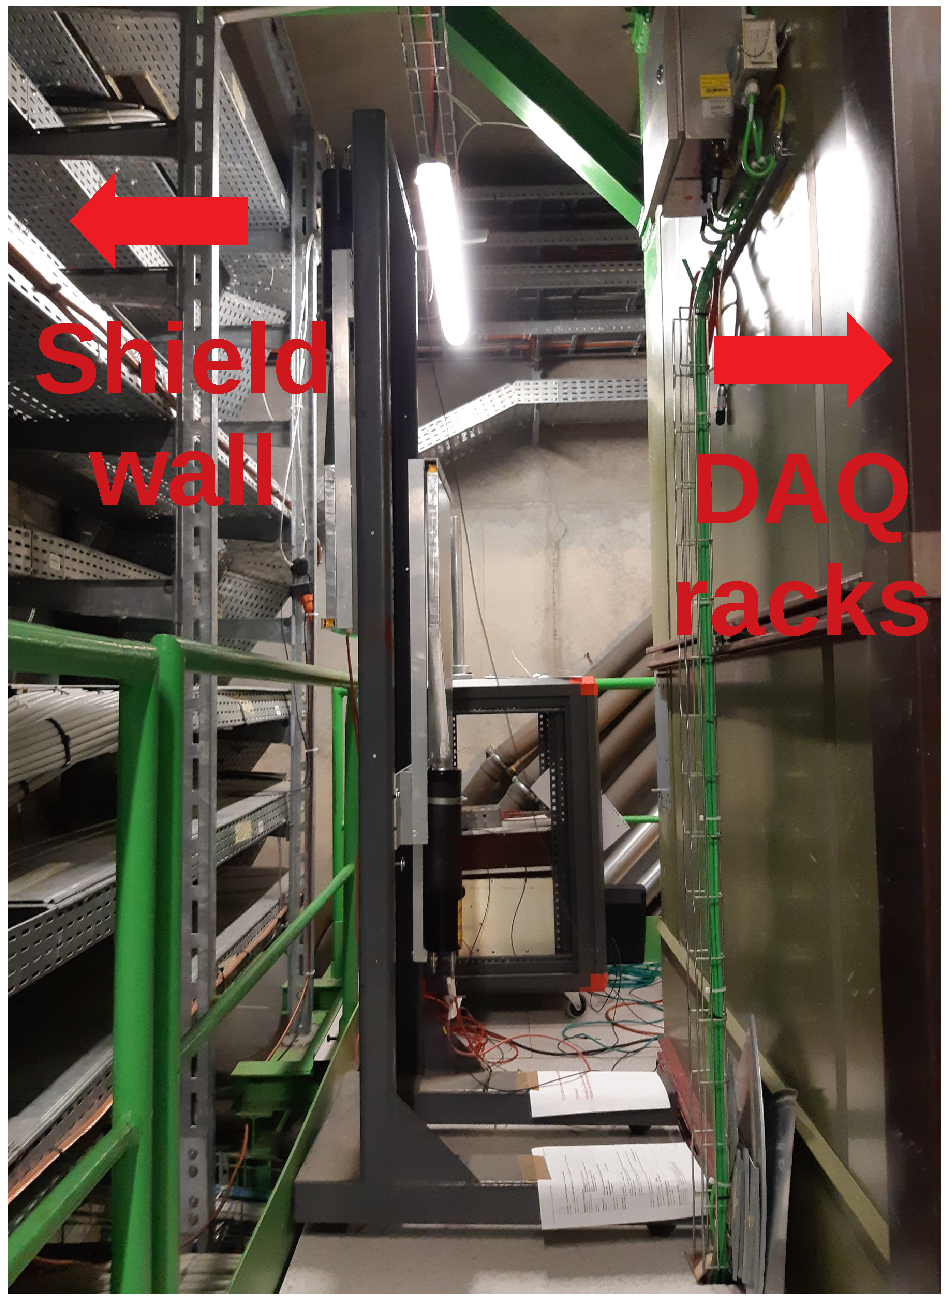
\includegraphics[width=0.5\textwidth]{figs/INT/Initial.pdf} &
%      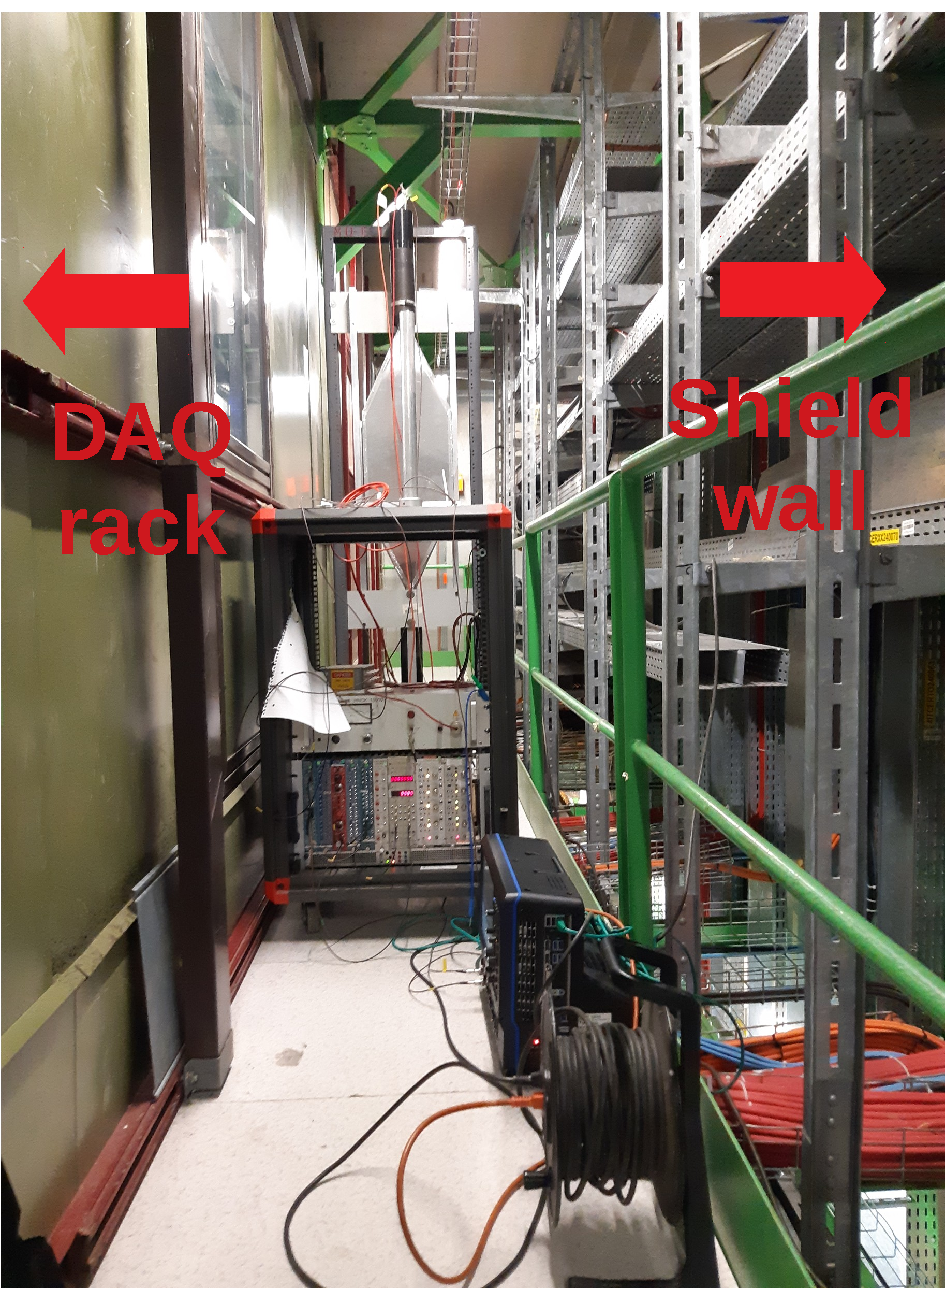
\includegraphics[width=0.5\textwidth]{figs/INT/Back_central.pdf} \\
%      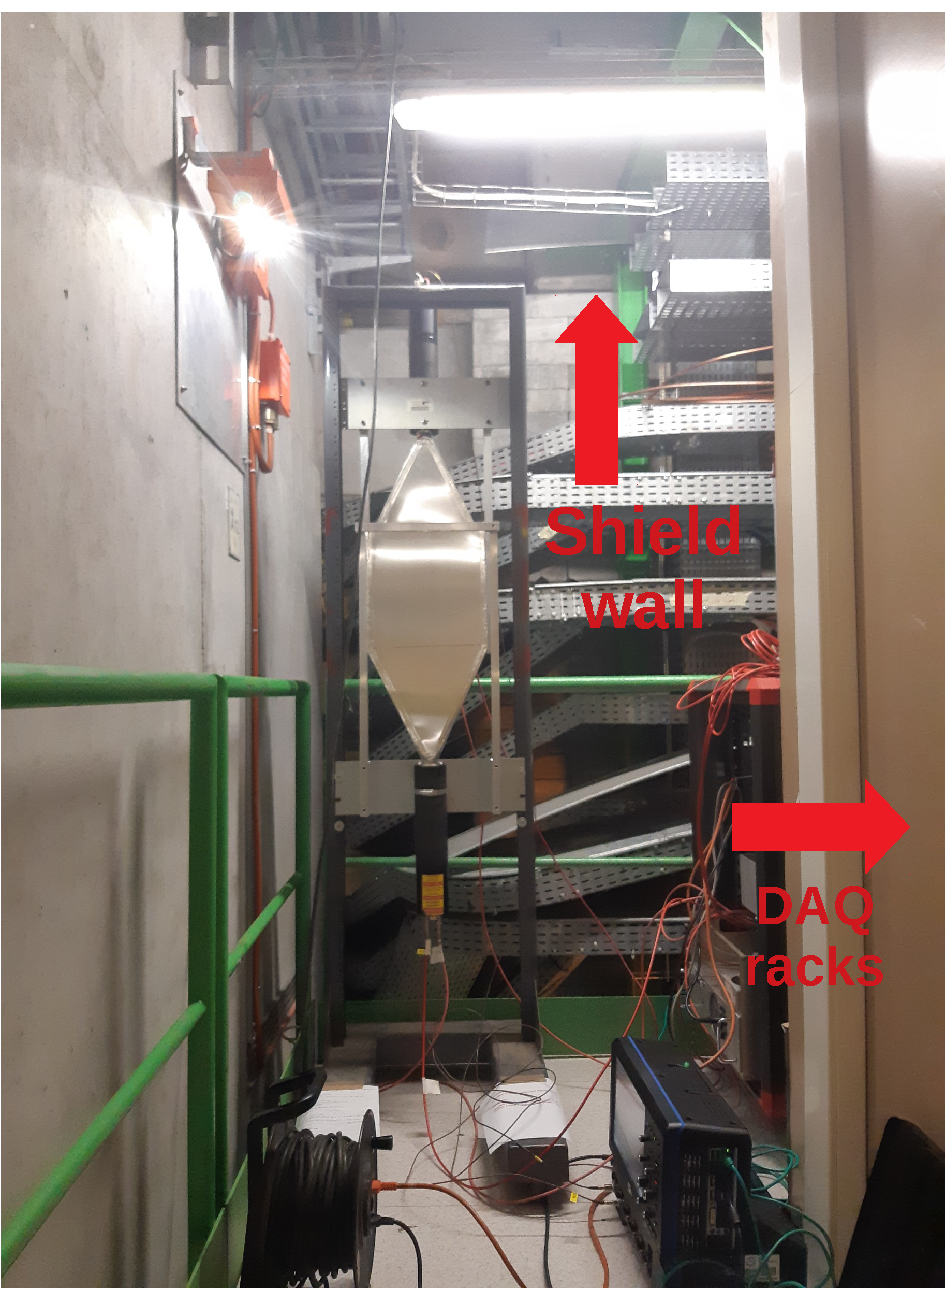
\includegraphics[width=0.5\textwidth]{figs/INT/Othercorner.pdf} &
%      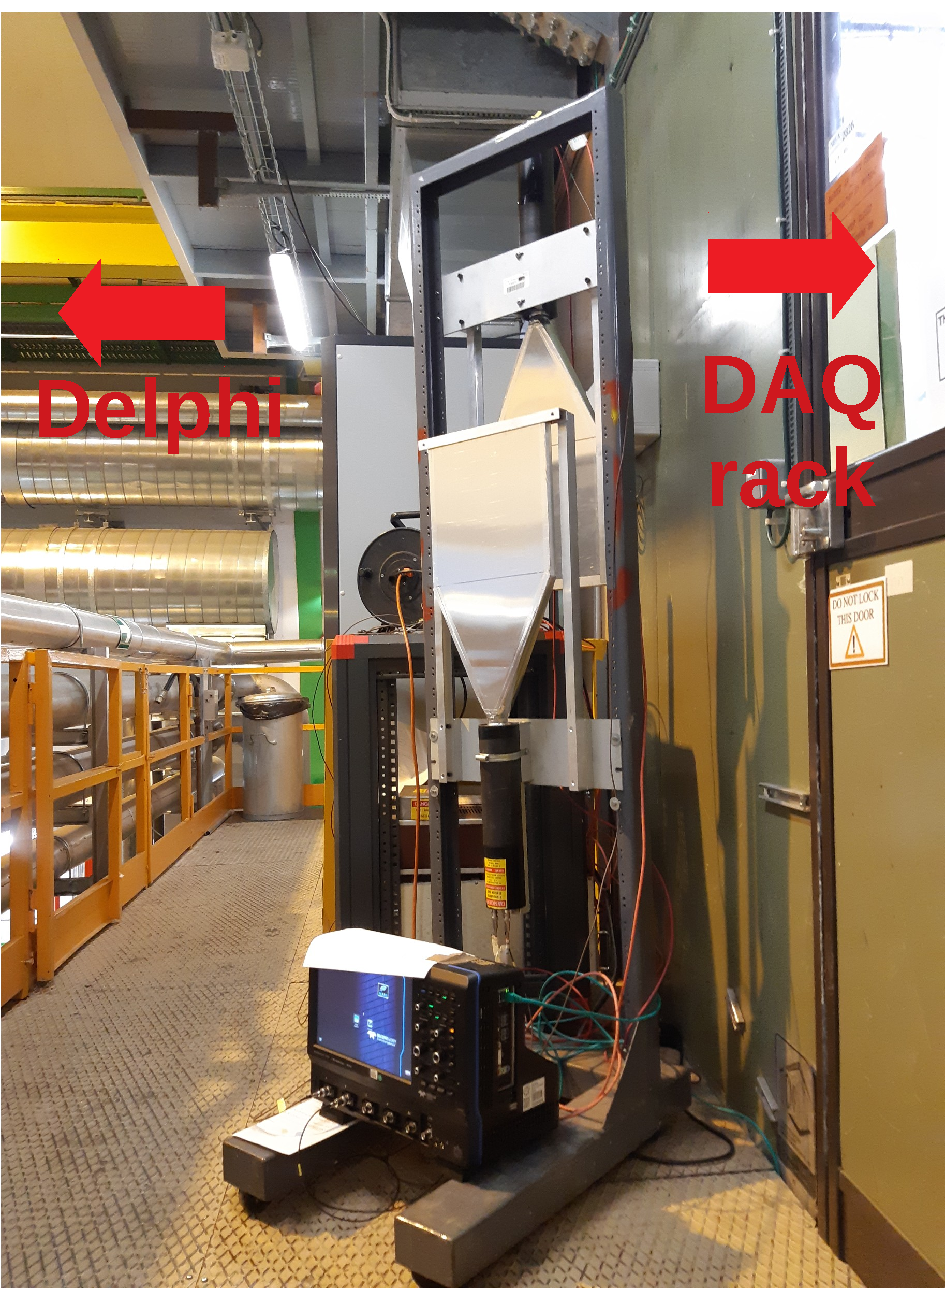
\includegraphics[width=0.5\textwidth]{figs/INT/D3_front.pdf} \\
%    \end{tabular}
%  \end{center}
%\caption{
%    Photos from each position at D3 platform
%}
%\end{figure}
